\subsection{QuaRot on the Attention Module}\label{sec:appx_attention_detailed}

Figure \ref{fig:attn_orig} shows the original attention module in large language models with RoPE. The input of the attention module is already rotated using the randomized Hadamard matrix $\mQ$ (see Section \ref{sec:method}) and in the first step, we fuse the inverse of such matrices into the input linear layers of the attention. In the next step, we fuse the exact Hadamard matrices on each block of the columns (proportional to each head) on the \texttt{V\_projection} layer to make sure that the Values will be rotated at the output of that layer. In the next step, we apply exact Hadamard transformations on the Keys and Queries and quantize the KV after RoPE operation (note that the Keys and Queries Hadmard transformations will be canceled during the attention operation). Finally, we apply another Hadamard transformation between heads before \texttt{Out\_projection} layer and fuse the inverse into the weights. Figure \ref{fig:attn_quarot} shows the result of applying QuaRot on the attention module.

\begin{figure}[h!]
    \centering
    \scalebox{0.8}{\begin{tikzpicture}[node distance=0.3cm and 0.6cm]  
    % Place nodes  
    \node (input) {\textbf{X}};  
    \node[nonlinearity, right=of input] (norm1) {$\frac{x}{\|x\|}$};  
    \node[block, right=of norm1] (norm2) {diag($\boldsymbol\alpha$)};
    \coordinate[right=of norm2] (split) {};
    \node[block, above right=of split, yshift=1.8em] (Wq) {$\textbf{W}_\textrm{q}$};
    \node[block, below right=of split, yshift=-1.8em] (Wv) {$\textbf{W}_\textrm{v}$};
    \node[block, right=of split] (Wk) {$\textbf{W}_\textrm{k}$};
    \node[nonlinearity, right=of Wq] (rope) {RoPE};
    \coordinate[right=of rope] (mha_in);
    \node[nonlinearity, right=of mha_in, align=center] (mha) {Multi-head\\Attention};
    \coordinate[right=of mha] (mha_right);

    \node[block, below right=of mha_right, yshift=-1.8em] (Wout) {$\textbf{W}_\textrm{out}$}; 
    \node[right= of Wout] (out) {\textbf{Y}};

    % KV cache
    \node[block, below= 4em of mha] (cache) {KV-cache};
      
    % Draw arrows  
    \draw[arrow] (input) -- (norm1);  
    \draw[arrow] (norm1) -- (norm2);
    \draw[thick] (norm2) -| (split);
    \draw[arrow] (split) |- (Wv);
    \draw[arrow] (split) |- (Wk);
    \draw[arrow] (split) |- (Wq);
    \draw[arrow] (Wq) -- (rope);
    \draw[thick] (rope) -- (mha_in);
    \draw[arrow] (mha_in) -- (mha);
    \draw[thick] (Wv) -| (mha_in);

    % k goes in and out of rope
    \coordinate (rope_k_in) at ($(rope.south west)!0.35!(rope.south east)$);
    \coordinate (rope_k_out) at ($(rope.south west)!0.65!(rope.south east)$);
    \draw[arrow] (Wk) -| (rope_k_in);
    \draw[arrow, dashed] (rope_k_out) |- (cache);

    \draw[thick] (mha) -- (mha_right);
    \draw[arrow] (mha_right) |- (Wout.west);
    \draw[arrow] (Wout) -- (out);

    % cache arrows
    \draw[arrow, dashed] (cache.north) -- (mha);
    \coordinate (start2) at ($(Wv.south east)!0.8!(Wv.north east)$);
    \draw[arrow, dashed] (start2) -- ($(cache.west|- start2)$);
    
    % Grouping nodes  
    \node[group, label=above:RMSNorm, fit=(norm1) (norm2)] {};  
    \node[group, label=above:Attention, fit=(split) (Wv) (Wk) (Wq) (mha) (Wout)] {};  
\end{tikzpicture}}
    \caption{Flow diagram of a self-attention block as used in most LMs, including the pre-positioned RMSNorm. Solid arrows represent flow during training, prefill and inference of each token. Dashed arrows show access to and from the KV cache, used at generation-time. The RoPE block computes relative positional embeddings. }
    \label{fig:attn_orig}
\end{figure}
%
\begin{figure}[h!]
    \centering
    \hspace*{-5mm}\scalebox{0.8}{\begin{tikzpicture}[node distance=0.3cm and 0.6cm]  
    % Place nodes  
    \node[label={[text=darkred]above:FP16}] (input) {$\mathbf{XQ}$};  
    \node[nonlinearity, right=of input] (norm1) {$\frac{x}{\|x\|}$};  
    \node[quant, text centered, text width=0.8em, right=of norm1] (quant1)  {\rotatebox{90}{quantize}};  
    \coordinate[right=3em of quant1] (split) {};
    \node[block, above right=of split, yshift=2.9em, label={[text=darkblue]above=-1em:INT4}] (Wq) {$\mathbf{Q}^\top(\boldsymbol\alpha)\mathbf{W}_\textrm{q}$};
    \node[block, below right=of split, yshift=-2.9em, label={[text=darkblue]above=-1em:INT4}] (Wv) {$\mathbf{Q}^\top\!(\boldsymbol\alpha)\mathbf{W}_\textrm{v}\mathbf{H}_\textrm{head}$};
    \node[block, right=of split, label={[text=darkblue]above=-1em:INT4}] (Wk) {$\mathbf{Q}^\top(\boldsymbol\alpha)\mathbf{W}_\textrm{k}$};
    \node[nonlinearity, right=2.5em of Wq] (rope) {RoPE};
    \coordinate[right=0.5em of rope] (mha_in);
    \node[nonlinearity, right=4.6em of mha_in, align=center] (mha) {Multi-head\\Attention};
    \coordinate[right=of mha] (mha_right);
    \node[quant, text centered, text width=0.8em, below right=of mha_right, yshift=-2.9em] (hadamard)  {\rotatebox{90}{hadamard heads}};  
    \node[quant, text centered, text width=0.8em, right=0.2em of hadamard] (quant2)  {\rotatebox{90}{quantize}};  
    \node[block, right=2em of quant2, label={[text=darkblue]above=-1em:INT4}] (Wout) {$\mathbf{H}\mathbf{W}_{\!\textrm{out}}\mathbf{Q}$}; 
    \node[right= of Wout, label={[text=darkred]above:FP16}] (out) {$\mathbf{YQ}$};

    % KV cache
    \node[block, below= 6.8em of mha, label={[text=darkblue]below=-1em:INT4}] (cache) {KV-cache};
    \node[quant, text centered, text width=0.8em, left=2em of cache] (hadamard_cache1)  {\rotatebox{90}{hadamard}};  
    \node[quant, text centered, text width=0.8em, right=0.2em of hadamard_cache1] (quant_cache1)  {\rotatebox{90}{quantize}};
    \node[quant2, text centered, text height=0.8em, above=0.2em of cache] (dequant)  {dequantize};  
    \node[quant2, text centered, text height=0.8em, above=0.2em of dequant] (hadamard_cache2)  {hadamard};  
    
      
    % Draw arrows  
    \draw[arrow] (input) -- (norm1);  
    \draw[arrow] (norm1) -- (quant1);
    \draw[thick] (quant1) -- (split) node[midway,above,text=darkblue] {INT4};
    \draw[arrow] (split) |- (Wv);
    \draw[arrow] (split) |- (Wk);
    \draw[arrow] (split) |- (Wq);
    \draw[arrow] (Wq) -- (rope) node[midway,above,text=darkred] {FP16};
    \draw[thick] (rope) -- (mha_in);
    \draw[arrow] (mha_in) -- (mha);
    \draw[thick] (Wv) -| (mha_in) node[pos=0.15,above,text=darkred] {FP16};

    % k goes in and out of rope
    \coordinate (rope_k_in) at ($(rope.south west)!0.35!(rope.south east)$);
    \coordinate (rope_k_out) at ($(rope.south west)!0.65!(rope.south east)$);
    \draw[arrow] (Wk) -| (rope_k_in) node[pos=0.16,above,text=darkred] {FP16};
    

    \draw[thick] (mha) -- (mha_right);
    \draw[arrow] (mha_right) |- (hadamard);
    \draw[arrow] (quant2) -- (Wout) node[midway,above,text=darkblue] {INT4};  
    \draw[arrow] (Wout) -- (out);

    % cache arrows
    \draw[arrow, dashed] (hadamard_cache2) -- (mha);
    \coordinate (start2) at ($(Wv.south east)!0.8!(Wv.north east)$);
    \draw[arrow, dashed] (start2) -- ($(hadamard_cache1.west|- start2)$);
    \draw[arrow, dashed] (rope_k_out) |- ($(hadamard_cache1.south west)!0.6!(hadamard_cache1.north west)$);
    
    % Grouping nodes  
    \node[group, label=above:RMSNorm, fit=(norm1) (quant1)] {};  
    \coordinate[above=0.99em of Wq] (dummy);
    \node[group, label=above:Attention, fit=(split) (Wv) (Wk) (Wq) (mha) (Wout) (dummy)] {};  
\end{tikzpicture}}
    \caption{QuaRot applied to an attention component. The RMSNorm scaling $\boldsymbol\alpha$ is absorbed into the input weight matrices, and the hidden state has been rotated by $\mQ$ in the same way as for the FFN block (see previous figure). Colored labels show the bit-width of each flow, and dashed lines show the flow to/from the KV cache. }
    \label{fig:attn_quarot}
\end{figure}



\subsection{Clipping Ratio Ablation}\label{sec:appx_clip_ratio}

We use the clipping ratio for both weights and activations during the quantization. During the weight quantization, we apply a linear search over the MSE error to extract the best clipping ratio for each column of the weight matrix. However, this is not possible as we quantize the inputs on the fly during the inference and we need to use a constant clipping ratio for such quantization.  We conclude that using 0.95 and 0.9 are suitable during asymmetric (KV cache) and symmetric (inputs) quantization which matches the finding from \citep{atom}.

\begin{table}[h]
\centering
\caption{WikiText perplexity of \llamaSmall with different clipping ratio. To study the effect of various clipping ratios, we keep the rest of the model in full precision.}
\vspace{1em}
\begin{tabular}{c|c|c|c|c}
% \toprule
 &  1.0 &  0.95 &  0.9 &  0.85 \\ \hline
Input Quantization & 5.938 & 5.910 & \textbf{5.828} & 5.850 \\ \hline
KV Cache Quantization & 5.513 & \textbf{5.510} & 5.517 & 5.532   \\ 
% \bottomrule
\end{tabular}
\label{tab:clipping_ratio_ablation}
\end{table}



\subsection{KV Cache Quantization Ablation}\label{sec:appx_kv_cach_quant}
We keep the rest of the model (including weights and activations) in high precision and apply our group-wise asymmetric quantization (with group-size 128) with various precision to keys and values. Table \ref{tab:kv_cache_quant_ablation} shows the results of using various precision during KV cache quantization. The results show a negligible (at most 0.21) perplexity degradation up to 3-bit KV cache (0.07 for \llamaBig model). In addition, by comparing the 3 and 4-bit quantization, we can see that compared to the values, keys are more sensitive to quantization as keeping the keys in 4-bits and values in 3-bits has 0.03 perplexity loss (0.18 for 3-bit keys and 4-bit values) on the \llamaSmall model. This matches the previous study on KV cache quantization \citep{kvquant, kivi}. The results show that using 3-bit KV-caches results in a better accuracy (5.68 on \llamaSmall model) compared to keeping the keys in 4-bits and quantizing the values using 2-bits (with 5.75 perplexity on \llamaSmall model).



\begin{table}[H]
    \centering
    \small
    \caption{
    \wiki perplexity with various KV cache precision using QuaRot.}
    \vspace{1em}
    \begin{tabular}{|c|c|ccc|}
        \toprule
        \textbf{K bits}&\textbf{V bits}&\multicolumn{3}{c|}{\textbf{\llama}}\\
        & &  \textbf{7B} & \textbf{13B} & \textbf{70B} \\
        \midrule
        16 & 16 &  5.47 & 4.88 & 3.32 \\
        \midrule
        4 & 4 &  5.51 & 4.91 & 3.33 \\
        4 & 3 &  5.54 & 4.93 & 3.35 \\
        4 & 2 &  5.75 & 5.09 & 3.43 \\
        3 & 4 &  5.65 & 5.01 & 3.38 \\
        3 & 3 &  5.68 & 5.02 & 3.39 \\
        3 & 2 &  5.93 & 5.21 & 3.48 \\
        2 & 4 & 8.06 & 6.42 & 3.89 \\
        2 & 3 & 8.18 & 6.50 & 3.92 \\
        2 & 2 &  9.23 & 7.07 & 4.13 \\
        \midrule
        
    \end{tabular}
    \vspace{5pt}
    \label{tab:kv_cache_quant_ablation}
\end{table}



\subsection{Weight-only Quantization Ablation}\label{sec:appx_weight_only_quant}

  QuaRot improves the quality of quantized models by removing the outlier features during the Hadamard transformations. As we fuse the Hadamard matrices into the weights, we study the role of these transformations for weight-only quantization (we keep the rest of the data-types in FP16). Table \ref{tab:ppl_weight_only} shows the \wiki perplexity results with asymmetric quantization. Using GPTQ quantization, QuaRot improves the perplexity by up to 2.65 in 4 bits. In addition, applying QuaRot improves the quality more in lower precision (2-3 bits) in all models. QuaRot also improves the RTN quantization up to 0.24 perplexity points. GPTQ still has a lower perplexity in 2-3 bits. However, applying QuaRot improves the quality of GPTQ in 2 bits to a non-trivial value (5.6 on the \llamaBig model).



\begin{table}[H]
    \centering

    \caption{
     Weight-only quantization results on \wiki on \llama models. We use asymmetric per-column quantization and keep the inputs and KV cache in FP16. We show the perplexity results >100 by Inf. We show the failed GPTQ experiments using NaN.}
    \vspace{1em}
\resizebox{\columnwidth}{!}{%
    \begin{tabular}{|c|ccc|ccc|ccc|}
        \toprule
        \multirow{2}{*}{\textbf{Method}}&\multicolumn{9}{c|}{\textbf{\llama}}\\
        &  \multicolumn{3}{c}{\textbf{7B}} & \multicolumn{3}{c}{\textbf{13B}} & \multicolumn{3}{c|}{\textbf{70B}} \\
        \midrule
        Baseline &  \multicolumn{3}{c|}{5.47}   & \multicolumn{3}{c|}{4.88}   & \multicolumn{3}{c|}{3.32}  \\
        \midrule
       \multicolumn{1}{|c}{}  &  A16W4 & A16W3 & A16W2  & A16W4 & A16W3 & A16W2  & A16W4 & A16W3 & A16W2  \\
        \midrule
       RTN & 6.99 &  Inf  &  Inf &  6.32 & Inf   & Inf & 4.45  & 42.11  &  Inf \\
       GPTQ & 8.25 &  NaN  &  NaN &  5.65 & 9.51   & Inf & 3.87  & 5.91  &  25.30 \\
       QuaRot-RTN & 6.76 & Inf   &  Inf & 5.48  & 48.89   & Inf &  3.66 & 5.25  & Inf  \\
       QuaRot-GPTQ & 5.60 & 6.09   & 22.07  & 5.00  &  5.37  & 10.41 & 3.41  & 3.72  & 5.60  \\
        \bottomrule
    \end{tabular}
   }
    \vspace{5pt}
    \label{tab:ppl_weight_only}
\end{table}



\subsection{Random Orthogonal Matrices Ablation}\label{sec:appx_random_orth_matrices}
QuaRot fuses Hadamard transformations into weight matrices to eliminate outliers. However, due to the computational  invariance property in LLMs, any 
orthogonal matrix can be fused to the model and we only need to apply an online $1\tfrac{1}{2}$ Hadamard transformations in each layer (see Section \ref{sec:method}). 
Here, we study the use of random orthogonal matrices in QuaRot. We start with a uniformly random matrix and apply QR decomposition to make it orthogonal before fusing it into the weights. 


\vspace{-2.5em}
\begin{table}[H]
    \centering
    \small
    \caption{
     \wiki perplexity of 4-bit QuaRot on \llama models with different orthogonal matrices.}
    \vspace{1em}
    \begin{tabular}{|c|ccc|}
        \toprule
        \multirow{2}{*}{\textbf{Method}}&\multicolumn{3}{c|}{\textbf{\llama}}\\
        & \textbf{7B} & \textbf{13B} & \textbf{70B} \\
        \midrule
        Baseline &  5.47   & 4.88   & 3.32  \\
        \midrule
       QuaRot (Random) & 7.45    &  5.84 & 4.07  \\
       QuaRot (Hadamard) &   6.10  & 5.40  & 3.79 \\
        \bottomrule
    \end{tabular}
    \vspace{5pt}
    \label{tab:random_orth_matrix}
\end{table}



Table \ref{tab:random_orth_matrix} shows the results of applying random orthogonal matrices 
on \llama models. Random orthogonal matrices are not as good as random Hadamard transformations and we have up 1.35 perplexity gap on \llamaSmall. 
However, as the model size increases, the gap decreases, resulting in a perplexity change of 0.28 in the \llamaBig model. Note that using the above matrices does not change the computation as we still use a fast Hadamard kernel for the down-projection and out-projection layers.




\subsection{Round-to-Nearest Weight Quantization: Detailed Results}\label{sec:appx_rtn_quant}

Table \ref{tab:rtn_results_detailed} shows the detailed results of QuaRot with GPTQ and round-to-nearest (RTN) weight quantization for both 6 and 8 bits on various tasks for \llama models.

\begin{table}[t]
    \centering
    \small
    \caption{\wiki Perplexity and zero-shot accuracy of QuaRot on the \llama family using 4, 6 and 8-bits with GPTQ and RTN weight quantization and RTN activation quantization.
    For zero-shot tasks, we use PIQA (PQ), WinoGrande (WG), HellaSwag (HS), Arc-Easy (A-e), Arc-Challenge (A-c), and LAMBADA (LA).The Precision column shows the bitwidth for all inputs, weights, and KV-caches.
    }
    \vspace{1em}
    \resizebox{\columnwidth}{!}{%
    \begin{tabular}{|c|c|c|c|ccccccc|}
        \toprule
        \textbf{Model} & \textbf{Method} & \textbf{Precision} & \textbf{PPL} $\downarrow$ & \textbf{PQ} $\uparrow$& \textbf{WG} $\uparrow$& \textbf{HS} $\uparrow$& \textbf{A-e} $\uparrow$& \textbf{A-c} $\uparrow$& \textbf{LA} $\uparrow$& \textbf{Avg.} $\uparrow$ \\
        \midrule
        \multirow{8}{*}{7B} & Baseline & FP16 & 5.47 & 79.11 & 69.06 & 75.99 & 74.58 & 46.25 & 73.90 & 69.82 \\
        \cmidrule{2-11}
         & \multirow{3}{*}{QuaRot-RTN}  & INT4 &  8.37 & 72.09 & 60.69 & 65.40 & 58.88 & 35.24 & 57.27 & 58.26 \\
         &   & INT6 &  5.56 & 78.73 & 67.80 & 75.92 & 74.16 & 46.08 & 73.86 & 69.42 \\
         &   & INT8 & 5.50 & 78.94 & 68.67 & 75.80 & 74.79 & 45.39 & 74.33 & 69.65 \\
         \cmidrule{2-11}
        & \multirow{3}{*}{QuaRot-GPTQ}  & INT4 & 6.10  & 76.77 & 63.77 & 72.16 & 69.87 & 40.87 & 70.39 & 65.64 \\
         &   & INT6 &  5.52 & 78.45 & 69.46 & 75.60 & 74.45 & 46.50 & 74.19 & 69.77 \\
         &   & INT8 &5.50 & 78.94 & 68.90 & 75.79 & 74.66 & 46.16 & 74.44 & 69.81\\
        \midrule
        
        \multirow{8}{*}{13B} & Baseline & FP16 & 4.88 & 80.47 & 72.22 & 79.39 & 77.48 & 49.23 & 76.75 & 72.59 \\
        \cmidrule{2-11}
        & \multirow{3}{*}{QuaRot-RTN}  & INT4 & 6.09  &  77.37 & 67.32 & 73.11 & 70.83 & 43.69 & 70.66 & 67.16 \\
         &  & INT6 & 4.95 & 79.65 & 72.22 & 79.10 & 77.27 & 50.34 & 76.75 & 72.56 \\
         &   & INT8 & 4.90 & 80.52 & 71.59 & 79.38 & 77.31 & 49.32 & 76.63 & 72.46 \\
         \cmidrule{2-11}
         & \multirow{3}{*}{QuaRot-GPTQ}  & INT4 &  5.40 &  78.89 & 70.24 & 76.37 & 72.98 & 46.59 & 73.67 & 69.79 \\
         &  & INT6 & 4.92 & 79.98 & 72.69 & 79.17 & 77.78 & 49.74 & 76.27 & 72.60 \\
         &   & INT8 &  4.90 & 80.36 & 71.98 & 79.38 & 77.31 & 49.15 & 76.79 & 72.49 \\
        \midrule
        
        \multirow{8}{*}{70B} & Baseline & FP16 & 3.32 & 82.70 & 77.98 & 83.84 & 80.98 & 57.34 & 79.58 & 77.07 \\
        \cmidrule{2-11}
        & \multirow{3}{*}{QuaRot-RTN}  & INT4 & 4.14  & 80.69 & 75.14 & 79.63 & 77.57 & 51.71 & 77.02 & 73.63 \\
         &   & INT6 & 3.36 & 83.24 & 77.90 & 83.47 & 80.93 & 58.28 & 79.41 & 77.21 \\
         &   & INT8 & 3.33 & 82.97 & 77.98 & 83.67 & 80.77 & 58.11 & 79.53 & 77.17 \\
         \cmidrule{2-11}
         & \multirow{3}{*}{QuaRot-GPTQ}  & INT4 &  3.79 &  82.43 & 76.24 & 81.82 & 80.43 & 56.23 & 78.73 & 75.98 \\
         &  & INT6 & 3.35 & 82.13  & 77.66  & 83.63 & 80.89 & 57.08  & 79.70  & 77.02 \\
         &   & INT8 & 3.33  & 83.13  & 78.06  & 83.72 & 80.85 & 58.19  & 79.72  & 77.28  \\
        \bottomrule
    \end{tabular}
    }
\label{tab:rtn_results_detailed}
\end{table}


\subsection{FP16 Hadamard Transformation Ablation}\label{sec:appx_had_fp16}

We use FP32 online Hadamard transformation across all our experiments.  Table \ref{tab:fp16_had_results} shows the results of using FP16 Hadamard transformation during the inference (for \textit{down-projection} and \textit{out-projection} layers). On \llamaSmall model, the results show <0.1 perplexity change on \wiki and <0.6\% averaged accuracy change on the zero-shot tasks, which we consider as noise. On \llamaMedium model, different Hadamard precisions have the same perplexities with 0.07\% difference in the averaged zero-shot results. We conclude that the model will not be changed using different Hadamard precision.


\begin{table}[H]
    \centering
    \small
    \caption{
    Ablation on the precision of online Hadamard transformations for QuaRot. We use \wiki perplexity as well as zero-shot tasks, explained in Section \ref{sec:ablation_study}.
    }
    \vspace{1em}
    \resizebox{\columnwidth}{!}{%
    \begin{tabular}{|c|c|c|c|ccccccc|}
        \toprule
        \multirow{2}{*}{\textbf{Model}} & \multirow{2}{*}{\textbf{Method}} & \textbf{Hadamard} & \multirow{2}{*}{\textbf{PPL} $\downarrow$} & \multirow{2}{*}{\textbf{PQ} $\uparrow$} & \multirow{2}{*}{\textbf{WG} $\uparrow$} &  \multirow{2}{*}{\textbf{HS} $\uparrow$} &\multirow{2}{*}{\textbf{A-e} $\uparrow$} & \multirow{2}{*}{\textbf{A-c} $\uparrow$} & \multirow{2}{*}{\textbf{LA} $\uparrow$} & \multirow{2}{*}{\textbf{Avg.} $\uparrow$} \\
        & & \textbf{Precision} & & & & & & & &  \\
        \midrule
        \multirow{4}{*}{7B} & Baseline & - & 5.47 & 79.11 & 69.06 & 75.99 & 74.58 & 46.25 & 73.90 & 69.82\\
        \cmidrule{2-11}
         & \multirow{2}{*}{QuaRot} & FP32 & 6.10  & 76.77 & 63.77 & 72.16 & 69.87 & 40.87 & 70.39 & 65.64 \\
         &   & FP16 & 6.08 & 76.99 & 66.46 & 72.59 & 69.07 & 41.21 & 70.59 & 66.21 \\
        \midrule
        \multirow{4}{*}{13B} & Baseline & - & 4.88 & 80.47 & 72.22 & 79.39 & 77.48 & 49.23 & 76.75 & 72.59 \\
        \cmidrule{2-11}
         & \multirow{2}{*}{QuaRot} & FP32 &5.40 &  78.89 & 70.24 & 76.37 & 72.98 & 46.59 & 73.67 & 69.79 \\
         &   & FP16 & 5.40 & 77.69 & 70.09 & 75.75 & 73.95 & 47.61 & 73.22 & 69.72 \\
        \bottomrule
    \end{tabular}
    }
\label{tab:fp16_had_results}
\end{table}


\subsection{\llamaIII Results}\label{sec:appx_llamaIII_acc}
In this section, we show the accuracy of applying QuaRot for quantizing the \llamaIIISmall and \llamaIIIBig models. Table \ref{tab:ppl_wikitext2_LLamaIII} shows the \wiki perplexity of quantizing the \llamaIII models with QuaRot using 4-bit quantization. Compared to Table \ref{tab:ppl_wikitext2}, we conclude that \llamaIII is more sensitive to quantization as we can see a higher gap between the quantized and FP16 models. Table \ref{tab:zero_shot_llamaIII} shows the accuracy results of those models on zero-shot tasks. 

\begin{table}[H]
    \centering
    \small
    \caption{
    \wiki perplexity results on 4-bit quantization of \llamaIII models with 2048 sequence length. 128G shows the group-wise quantization with group size 128.}
    \vspace{0.5em}
    \resizebox{.6\textwidth}{!}{
    \begin{tabular}{|c|c|c|cc|}
        \toprule
        \multirow{2}{*}{\textbf{Method}}&\textbf{Weight}&\textbf{\#Outlier}&\multicolumn{2}{c|}{\textbf{\llamaIII}}\\
        &  \textbf{Quantization} & \textbf{Features} & \textbf{8B} & \textbf{70B} \\
        \midrule
        Baseline &  -  & - & 6.14 & 2.86 \\
        \midrule
       \multirow{1}{*}{QuaRot}  &   GPTQ & 0 & 8.16 & 6.66 \\ 
        \midrule
        QuaRot-128G & GPTQ-128G  & 0 &  7.36 & 5.51 \\ 
        \bottomrule
    \end{tabular}
    }
    %\vspace{5pt}
    \label{tab:ppl_wikitext2_LLamaIII}
\end{table}

\begin{table}[H]
    \centering
    \small
    \caption{Zero-shot accuracy of \llamaIII models with 4-bit QuaRot on PIQA (PQ), WinoGrande (WG), HellaSwag (HS), Arc-Easy (A-e), Arc-Challenge (A-c), and LAMBADA (LA).}
    \vspace{0.5em}
    \resizebox{.8\textwidth}{!}{
    \begin{tabular}{|c|c|cccccc|c|}
        \toprule
        \textbf{Model} & \textbf{Method} & \textbf{PQ} & \textbf{WG} & \textbf{HS} & \textbf{A-e} & \textbf{A-c} & \textbf{LA} & \textbf{Avg.} \\
        \midrule 
        \multirow{2}{*}{\llamaIIISmall} & FP16& 80.74  & 72.77  &79.06  &77.82  &53.33  &75.63  &73.22  \\
         & QuaRot& 75.14  & 65.82  & 72.94  &68.01  &43.34  &65.81  &65.18  \\
        \bottomrule  
        \multirow{2}{*}{\llamaIIIBig} & FP16& 84.66  & 80.51  &84.89  &85.86  & 64.25 & 79.47  &79.94  \\
         & QuaRot& 78.07  & 69.30  &77.33  &73.44  &47.53  &69.57  &69.21  \\
        \bottomrule  
    \end{tabular}
    }
\label{tab:zero_shot_llamaIII}
\end{table}

\subsection{Phi-3-mini-4k-instruct Results}\label{sec:appx_phi3_acc}
In this section, we show the accuracy of applying QuaRot for quantizing the Phi-3-mini-4k-instruct model~\citep{abdin2024phi3}. Table \ref{tab:rtn_results_detailed_phi3} shows the accuracy results of the model in terms of perplexity and on zero-shot tasks. 

\begin{table}[!h]
    \centering
    \small
    \caption{\wiki Perplexity and zero-shot accuracy of QuaRot on the Phi-3-mini-4k-instruct model (revision = ff07dc01) using 4, 6 and 8-bits with GPTQ and RTN weight quantization and RTN activation quantization.
    For zero-shot tasks, we use PIQA (PQ), WinoGrande (WG), HellaSwag (HS), Arc-Easy (A-e), Arc-Challenge (A-c), and LAMBADA (LA).
    }
    \vspace{1em}
    \resizebox{\columnwidth}{!}{%
    \begin{tabular}{|c|c|c|c|ccccccc|}
        \toprule
        \textbf{Model} & \textbf{Method} & \textbf{Precision} & \textbf{PPL} $\downarrow$ & \textbf{PQ} $\uparrow$& \textbf{WG} $\uparrow$& \textbf{HS} $\uparrow$& \textbf{A-e} $\uparrow$& \textbf{A-c} $\uparrow$& \textbf{LA} $\uparrow$& \textbf{Avg.} $\uparrow$ \\
        \midrule
        \multirow{8}{*}{Phi-3-mini} & Baseline & FP16 & 6.35 & 80.47 & 73.72 & 78.45 & 80.13 & 57.51 & 68.37 & 73.11 \\
        \cmidrule{2-11}
         & \multirow{3}{*}{QuaRot-RTN}  & INT4 &  11.69 & 68.39 & 58.64 & 60.60 & 65.87 & 39.25 & 43.99 & 56.12 \\
         &   & INT6 & 6.78 & 79.54 & 73.01 & 77.46 & 79.21 & 55.12 & 67.53 & 71.98 \\
         &   & INT8 & 6.58 & 79.71 & 74.11 & 78.63 & 80.47 & 56.66 & 68.56 & 73.02 \\
         \cmidrule{2-11}
        & \multirow{3}{*}{QuaRot-GPTQ}  & INT4 & 7.85  & 75.35 & 67.88 & 72.95 & 72.98 & 48.12 & 60.78 & 66.34 \\
         &   & INT6 & 6.63 & 79.54 & 72.69 & 78.50 & 79.42 & 56.74 & 68.85 & 72.67 \\
         &   & INT8 & 6.58 & 80.25 & 74.19 & 78.54 & 80.35 & 57.08 & 68.64 & 73.18 \\
        \bottomrule
    \end{tabular}
    }
\label{tab:rtn_results_detailed_phi3}
\end{table}


\subsection{Performance Analysis}\label{sec:appx_performance_analysis}

 We implement the attention mechanism using three routines: 1) \textbf{Init}: During the prefill stage, this routine initializes the cache from all the key and value vectors in the prefill. The attention output during prefill is computed directly using Flash Attention \citep{flash-attention} since we already have access to dequantized keys and values. 2) \textbf{Append}: During decoding, this routine is called first to quantize the current keys and values and append them to the cache. 3) \textbf{Decode}: Finally, this routine is called during decoding with the current query vector. The routine computes the attention output using a quantized implementation of flash attention which can load the quantized cache and compute the final value vector. 

\paragraph{4-bit Linear and Attention Layers.} We benchmark our 4-bit linear layer which involves 4-bit matrix multiplication. For a given input of FP16, the layer optionally computes the Hadamard operation, then calls the quantization kernel to quantize and save the input in a sub-byte format. In the next step, the quantized weights and input are passed to the \texttt{CUTLASS} 4-bit GEMM kernel. Finally, the output is dequantized and cast back to FP16. Figure \ref{fig:linear_timing} shows the speedup of our 4-bit layer for different layer sizes where the layer sizes match the FFN linear layer sizes in \llama models. Our 4-bit linear layer gets 3.2x speedup relative to FP16 in the \llamaSmall model, and 4.3x on the \llamaBig model. These numbers are for a batch size of 1, we find that scaling is approximately linear with batch size: more results in Table \ref{tab:Qlinear_bench}. We include the runtime with and without Hadamard operations, as $\mW_\textrm{up}$ and $\mW_\textrm{gate}$ do not require Hadamard transforms, whilst $\mW_\textrm{down}$ does. We see that the Hadamard transform adds very little overhead to the forward pass at most 7\% overhead.

\begin{figure}
    \centering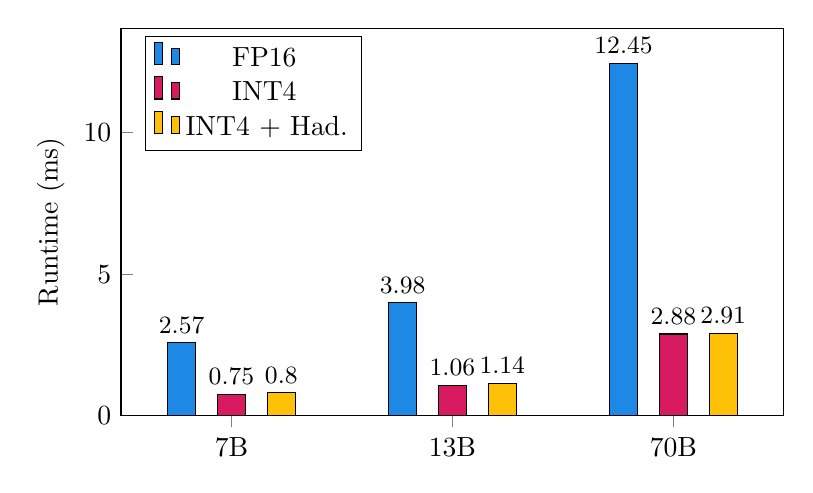
\begin{tikzpicture}  
\definecolor{col1}{HTML}{1E88E5}
\definecolor{col2}{HTML}{D81B60}
\definecolor{col3}{HTML}{FFC107}

\begin{axis}[
    width=10cm, 
    height=6.5cm,  
    ybar=8pt,  
    enlarge x limits=0.25,  
    legend style={at={(0.2,0.98)},  
      anchor=north},  
    ylabel={Runtime (ms)},
    symbolic x coords={7B, 13B, 70B},  
    xtick=data,  
    nodes near coords,  
    nodes near coords align={vertical},  
    nodes near coords style={font=\small},
    ymin = 0,
    ytick pos=left,
    xtick pos=left,
    ]  
\addplot[fill=col1] coordinates {(7B, 2.569) (13B,3.983)  (70B, 12.45)};
\addplot[fill=col2] coordinates {(7B,0.749) (13B,1.063) (70B,2.881)}; 
\addplot[fill=col3] coordinates {(7B,0.798) (13B,1.142) (70B,2.911)}; 
\legend{FP16\,, INT4\,, INT4 + Had.}  
\end{axis}  
\end{tikzpicture}  
  


    \caption{\label{fig:linear_timing} Performance of 16-bit and 4-bit linear layer for 2048 sequence lengths with and without online Hadamard transformation on a NVIDIA RTX 3090 GPU, averaged over 1000 runs. The matrix sizes correspond to the linear layer sizes in \llama FFN blocks (i.e. $\mW_\textrm{down}$). Here the batch size is 1, but the performance ratio holds for larger batches (see Table \ref{tab:Qlinear_bench}).}
\end{figure}



We also compare the speed of performing append and decode routines for a single token given a cache of size 2047. This is equivalent to the cost of decoding the 2048-th token in a sequence. The comparison between the speed of FP16 and INT4 for different batch sizes and layer sizes is reported in Table~\ref{tab:QAttention_bench}. For the layer size used in \llamaSmall, our 4-bit implementation gets up to 1.72x improvement in speed for the larger batch sizes (e.g. from 16 onwards). The 4-bit cache is slower than FP16 for smaller batch sizes (e.g. up to 8). Note that this is intuitive as the main benefit of the 4-bit cache is reducing the I/O cost. A speed up is only visible if this reduction is more significant than the quantization overhead which happens for either larger batch sizes or longer sequences. 




Table \ref{tab:Qlinear_bench} shows the results of benchmarking our 4-bit linear layer. The layer sizes are extracted based on the linear layer sizes in \llama models (for out-projection and down-projections). We apply both FP16 and FP32 Hadamard transformations and show the runtime on NVIDIA RTX GPU using 2048 sequence lengths. Table \ref{tab:QAttention_bench} shows the results of decoding a single token in the attention layer when we apply KV-cache quantization. We extract the size of the attention layer based on the \llama models. 


 \begin{table}[t]
    \centering
    \begin{tabular}{c|c|c|c|c|c}
\toprule
Layer Size & Batch Size  &  FP16 & INT4 & INT4 + FP32  Had & INT4 + FP16 Had\\
\midrule
\multirow{6}{*}{4096x4096} &   1 & 1.043 & 0.370 & 0.409 & 0.403\\
& 2 & 1.902 & 0.696 & 0.790 & 0.789\\
 &  4 & 3.715 & 1.361 & 1.522 & 1.529\\
 &  8 & 7.200 & 2.675 & 2.999 & 3.011\\
 &  16 & 14.508 & 5.357 & 5.973 & 5.976\\
 &  32 & 29.029 & 10.641 & 11.900 & 11.911\\
\midrule
\multirow{6}{*}{5120x5120} & 1 & 1.418 & 0.464 & 0.552 & 0.547\\
& 2 & 2.918 & 0.937 & 1.100 & 1.097\\
 &  4 & 5.852 & 1.888 & 2.206 & 2.207\\
 & 8 & 11.465 & 3.809 & 4.428 & 4.422\\
 &  16 & 22.807 & 7.547 & 8.755 & 8.759\\
 & 32 & 45.312 & 15.019 & 17.417 & 17.440\\
 \midrule
\multirow{6}{*}{8192x8192} &  1 & 3.696 & 0.997 & 1.084 & 1.083\\
& 2 & 7.191 & 1.944 & 2.099 & 2.099\\
 & 4 & 14.236 & 3.918 & 4.208 & 4.207\\
 & 8  & 28.508 & 7.944 & 8.460 & 8.415\\
 &  16 & 57.814 & 15.793 & 16.859 & 16.871\\
 & 32 & 115.462 & 31.693 & 33.780 & 33.791\\
 \midrule
\multirow{6}{*}{11008x4096} &  1 & 2.569 & 0.749 & 0.798 & 0.801\\
& 2 & 5.027 & 1.478 & 1.555 & 1.558\\
& 4 & 9.752 & 2.990 & 3.140 & 3.144\\
 & 8 & 19.696 & 6.031 & 6.296 & 6.306\\
 &  16 & 38.883 & 11.978 & 12.503 & 12.527\\
 &  32 & 78.320 & 23.874 & 24.935 & 24.974\\
 \midrule
\multirow{6}{*}{13824x5120} & 1 & 3.983 & 1.063 & 1.142 & 1.139\\
& 2 & 7.869 & 2.148 & 2.291 & 2.293\\
 & 4 & 15.410 & 4.340 & 4.616 & 4.614\\
 & 8 & 30.761 & 8.719 & 9.231 & 9.240\\
&  16 & 61.203 & 17.318 & 18.345 & 18.343\\
 &  32 & 122.926 & 34.816 & 36.953 & 36.940\\
 \midrule
\multirow{6}{*}{28672x8192} &1 & 12.450 & 2.881 & 2.911 & 2.911\\
& 2 & 25.391 & 5.828 & 5.892 & 5.896\\
& 4 & 50.742 & 11.938 & 11.947 & 11.976\\
& 8 & 101.290 & 24.186 & 24.202 & 24.216\\
&  16 & 202.909 & 48.238 & 48.325 & 48.356\\
& 32 & 406.344 & 96.761 & 97.044 & 96.892\\
\bottomrule
\end{tabular}
\vspace{0.5em}
    \caption{Performance of 4-bit linear layer for 2048 sequence lengths with and without online Hadamard transformation on a NVIDIA RTX 3090 GPU. The matrix sizes correspond to the linear layer sizes in \llama models. We averaged over 100 runs and report the numbers in milliseconds.
    }
    \label{tab:Qlinear_bench}
\end{table}



\clearpage
 \begin{table}[H]
    \centering
    \begin{tabular}{c|c|c|c|c|c}
\toprule
head\_num x head\_dim & Batch Size  &  FP16 & INT4 & INT4 + FP32  Had & INT4 + FP16 Had\\
\midrule
\multirow{5}{*}{32x128} &    1 & 0.713 & 1.033 & 1.163 & 1.117\\
& 2 & 0.723 & 1.035 & 1.168 & 1.122\\
 &    4 &  0.781 & 1.033 & 1.168 & 1.118\\
 &    8 &   0.984 & 1.042 & 1.173 & 1.126\\
 &    16 & 1.348 & 1.018 & 1.153 & 1.102\\
 &    32 & 2.098 & 1.168 & 1.247 & 1.216\\
\midrule
 \multirow{5}{*}{40x128} &    1 & 0.712 & 1.026 & 1.157 & 1.106\\
 & 2 & 0.726 & 1.035 & 1.173 & 1.121\\
 &    4 & 0.831 & 1.038 & 1.166 & 1.115\\
 &    8 & 1.065 & 1.048 & 1.181 & 1.128\\
 &    16 & 1.525 & 1.021 & 1.153 & 1.102\\
 &    32 & 2.480 & 1.244 & 1.320 & 1.287\\
 \midrule
 \multirow{5}{*}{64x128} &    1 &0.715 & 1.028 & 1.160 & 1.108\\
 & 2 & 0.780 & 1.034 & 1.171 & 1.117\\
 &    4 &  0.984 & 1.034 & 1.171 & 1.120\\
 &    8 & 1.361 & 1.048 & 1.182 & 1.130\\
 &    16 & 2.071 & 1.147 & 1.223 & 1.192\\
 &    32 & 3.563 & 1.566 & 1.645 & 1.612\\
\bottomrule
\end{tabular}
\vspace{0.5em}
    \caption{Performance of decoding a single token with 4-bit KV cache for the attention layer for 2048 sequence lengths with and without online Hadamard transformation on an NVIDIA RTX 3090 GPU. We evaluate generating the last token when the 2047 tokens are already cached in the attention.  We extract the number of heads (head\_num) and their dimensions (head\_dim) based on different \llama models. We averaged over 100 runs to report the numbers in milliseconds.
    }
    \label{tab:QAttention_bench}
\end{table}


Tables \ref{tab:transformer_layer_speedup} and \ref{tab:peak_memory} show the detailed speedups and memory saving of a single transformer block for QuaRot on \llamaSmall model using NVIDIA RTX 3090 GPU.

\begin{table}[H]
 
    \centering
    \begin{tabular}{|c|c|c|c|c|}
    
\toprule
  Model & Batch Size  & Speedup \\
\midrule
 \multirow{5}{*}{\llamaSmall} &1 & 1.97$\times$ \\
&4 & 2.06$\times$ \\
&16 & 2.11$\times$ \\
&32 & 2.14$\times$ \\
&64 & 2.16$\times$ \\
\midrule
 \multirow{4}{*}{\llamaBig} &1 &  3.16$\times$ \\
&4 &  3.27$\times$ \\
&16 &  3.32$\times$ \\
&32 &  3.33$\times$ \\
\bottomrule
\end{tabular}
\vspace{0.5em}
    \caption{
    Time-to-first-token (prefill) speedup of each transformation block of \llama models in QuaRot (over the FP16 model) on NVIDIA RTX 3090 GPU. We use 2048 sequence lengths with different batch sizes.
    }
    \label{tab:transformer_layer_speedup}
\end{table}

\begin{table}[H]

    \centering
    \begin{tabular}{|c|c|c|c|c|c|}
\toprule
\multirow{2}{*}{Model} & Batch & Sequence & Baseline & QuaRot & Saving \\
  & Size  &  Length & (GB) & (GB) &  Factor  \\
\midrule
\multirow{10}{*}{\llamaSmall} &
\multirow{4}{*}{1} & 256  & 0.392GB  & 0.108GB  & 3.63$\times$ \\
 & & 512  & 0.396GB &  0.108GB &  3.66$\times$ \\
 & & 1024  &  0.404GB   & 0.110GB  &  3.66$\times$ \\
 & & 2048  & 0.419GB & 0.114GB &  3.67$\times$     \\
 & & 4096 & 0.451GB  & 0.125GB  &  3.60$\times$ \\ \cmidrule{2-6}
& \multirow{4}{*}{16} & 256  & 0.464GB &0.128GB  &  3.63$\times$ \\ 
 & & 512  & 0.528GB  &0.144GB  &  3.66$\times$ \\
 & & 1024  &  0.655GB  & 0.177GB &  3.70$\times$ \\
 & & 2048  & 0.908GB   & 0.244GB  &  3.72$\times$ \\
 & & 4096 & 1.416GB  &  0.378GB &  3.75$\times$ \\
 \midrule
\multirow{10}{*}{\llamaBig} &
\multirow{4}{*}{1} & 256  & 1.605GB & 0.409GB   &  3.92$\times$ \\
 & & 512  & 1.606GB &  0.409GB &  3.92$\times$ \\
 & & 1024  &  1.608GB   &  0.410GB & 3.92$\times$ \\
 & & 2048  & 1.612GB & 0.411GB &  3.92$\times$     \\
 & & 4096 & 1.620GB  &  0.413GB &  3.92$\times$ \\ \cmidrule{2-6}
& \multirow{4}{*}{16} & 256 & 1.626GB &  0.418GB & 3.89$\times$ \\ 
 & & 512  & 1.642GB  &0.422GB  &  3.89$\times$ \\
 & & 1024  &  1.674GB  & 0.430GB &  3.89$\times$ \\
 & & 2048  &  1.738GB  & 0.447GB  &  3.89$\times$ \\
 & & 4096 & 1.865GB  & 0.480GB  &  3.89$\times$ \\
\bottomrule
\end{tabular}
\vspace{0.5em}
    \caption{
    Peak Memory usage (in GB) for decoding a single token on a single transformation block of \llama models with KV caches of different lengths and with different batch size. 
    }
    \label{tab:peak_memory}


\vspace{-1.5em}
\end{table}
